\chapter{Accuracy evaluation and analysis}
Measurement accuracy is among the most crucial benchmarks to judge worth of a metrology equipment. To assess measurement accuracy of the developed system the problem can be viewed as having three components as even the structure of this thesis suggests:System calibration, stereo-correspondence computation and triangulation. Hence it was decided to perform assessments of accuracy of each of these individual components. However scope of this work is limited to accuracy evaluation of stereo-correspondence and system calibration only because these components decide the accuracy of optical triangulation as can be implied from equations 4.7,4.8. Hence the accuracy of optical triangulation method cannot be studied completely isolated from that of stereo-correspondence and system calibration unless both correspondence and calibration estimates are kept fixed.\newline

This chapter is logically divided into two parts. First part covered by sections 5.1 and 5.2 will describe the experiments performed to assess the measurement accuracy and precision of the system developed and further compares it with the nowadays popular 3D sensor \textit{Microsoft Kinect}. This comes under \textit{accuracy evaluation}. Second part covered in sections 5-3 and 5-4 further delves deeper into quantitative assessment of \textit{independent} individual components of the developed system namely system calibration and stereo-correspondence module. This comes under \textit{accuracy analysis}. Coded phase-shift scanner will be abbreviated by \textit{CPSS} in this chapter.


\section{Evaluation of accuracy and precision of developed system}
For evaluating the measurement accuracy and precision 3D reconstruction of a planar surface was used. For visualization of point clouds Point cloud library[53] was used. Before describing experimental procedures and results each term will be described for clarity in equations 5-1 and 5-2. Same definition was used for comparative evaluation of developed system with Kinect in section 5.2 and hence will not be repeated there.
\paragraph{Precision.}
\label{def:precision}
It refers to the percentage deviation of measurements from their mean value however it should be noted that precision does not imply accuracy[54]. Higher the percentage deviation lower the measurement precision. It is a measure of \textit{uncertainty} in the measurement. The definition used in this work is:-\newline


\begin{equation}
Precision=\frac{\sum_{p=1}^{vp}\Bigg[\frac{\sum_{i=1}^{vs_{p}}\Bigg[\frac{mean_{p}-sample_{i}}{mean_{p}+1}\Bigg]}{vs_{p}}\Bigg]}{vp}
\end{equation}

\noindent
where \textit{p} is the index of pixel number and \textit{vp} denotes total \textit{valid} pixels \footnote{\textbf{CPSS}:Generally thresholding at the edge of strips in the captured binary coded patterns is \indent \indent ambiguous due to a grey region at such regions instead of unambiguous black or white hence \indent \indent these pixels are considered as \textit{invalid}.\newline
\indent \indent \textbf{Kinect}:Pixels with NaN's in any of corresponding estimated X, Y or Z coordinates are \indent \indent \textit{invalid}.} in an image, \textit{mean\textsubscript{p}}\footnote{$mean_p=\frac{\sum_{i=1}^{vs_{p}}\big[sample_{i}\big]}{vs_{p}}$} is the mean X/Y/Z value of 3D point corresponding to pixel \textit{p}. \textit{sample\textsubscript{i}} is the corresponding X/Y/Z value of sample \textit{i}, \textit{vs\textsubscript{p}} is the total valid samples for pixel \textit{p}. To avoid divide-by-zero \textit{mean+1} has been used.


\paragraph{Measurement accuracy.}
\label{def:accuracy}
It refers to the percentage deviation of a measurement from its actual value. Higher the deviation lower the accuracy. The definition used in this work is:


\begin{equation}
Accuracy=\frac{\sum_{i=1}^{N}\Bigg[\frac{Actual_{i}-measured_{i}}{Actual_{i}}\Bigg]}{N}
\end{equation}

\noindent
where \textit{N} is total number of measured lengths, \textit{Actual\textsubscript{i}} is the actual value for i\textsuperscript{th} measured length, similarly \textit{measured\textsubscript{i}} is the corresponding average measured length.


\subsection{Precision}
\label{experiment:precision}
To assess precision(or uncertainty), a planar surface was scammed 10 times for 5 depth levels. For each depth, the percentage average absolute deviation was computed for the 3D-coordinates returned by system corresponding to each pixel with respect to mean of measurements at that pixel, and averaged it over the complete image to get the percentage average absolute deviation at that depth. Table 5-1 shows the variation of \% average absolute deviation of X,Y,Z component measurements with depth.
\begin{table}[ht]
% table caption is above the table
\centering
\label{tab:1}       % Give a unique label
% For LaTeX tables use
\begin{tabular}{c c c c}
\hline\noalign{\smallskip}
Distance & X\% & Y\% & Z\% \\
\noalign{\smallskip}\hline\noalign{\smallskip}
1.3 & 0.006 & 0.010 & 0.007 \\
1.6 & 0.015 & 0.019 & 0.037\\
1.9 & 0.010 & 0.024 & 0.050 \\
2.2 & 0.014 & 0.029 & 0.094\\
2.5 & 0.010 & 0.025 & 0.141 \\
\noalign{\smallskip}\hline
\end{tabular}
\caption{CPSS:Precision along X,Y,Z axes}
\end{table}

\subsection{Measurement accuracy}
\label{experiment:accuracy} 
To assess the dependence of measurement accuracy on distance of object from sensor it was decided to determine error in length measurements. Specifically, a planar-face of a box was used with a checkerboard attached to it. Figure~\ref{fig:experiment_setup} shows the overall setup for measurement. Using checkerboard detection[55] the image coordinates of 4 outermost corners were determined and 6 3D distances (4 edges and 2 diagonals) were measured using corresponding 3D coordinates in the point cloud. Object was scanned the 10 times for each depth and the average measured lengths from these scans were calculated. It should be pointed out that the depth range was limited by the depth of field of camera-projector system. Although phase shift technique suffers from non-linearity of projector and camera  system and needs to have gamma correction[7], measurements were performed on raw point cloud without any correction/enhancement to get upper bounds on accuracy of the CPSS implementation. Figure~\ref{fig:experiment_plot} shows the orientations and distances used in measurement experiments. This figure shows position of each view of measurement object used for evaluating measurement accuracy. Individual views are indexed as \textit{\#id} where \textit{id} is the number of view. Further, relative position and orientation of developed system and Kinect(described in next section) are shown. The apparent curved path for the positions used for measurement(see figure~\ref{fig:experiment_plot}) ensured that measurement object remains in common field-of-view of both camera and projector of CPSS system. 

\begin{figure}[ht]
\centering
\includegraphics[width=10cm,height=8cm]{../img_source/setup.jpg}
\caption{Experiment setup}
\label{fig:experiment_setup}
\end{figure}


\begin{figure}[ht]
\centering
\includegraphics[width=17cm,height=15cm]{../img_source/experiment_plot.jpg}
\caption{Orientations and positions used for experiments}
\label{fig:experiment_plot}
\end{figure}


Table 5.2 summarizes the observed dependence of measurement accuracy on distance. Whereas in Table 5.3 measurement uncertainty is shown which is the average \% relative deviation of 10 measurements with respect to their mean value. It should be noted that measurement uncertainty is a measure of random error as it is calculated from individual measurements rather than from an averaged dataset. 

\begin{table}[ht]
\centering
\label{table:accuracy}
\begin{tabular}{c c}
\hline\noalign{\smallskip}
Distance & CPSS(\% error) \\
\noalign{\smallskip}\hline\noalign{\smallskip}
1.3 & 1.153  \\
1.6 & 0.744    \\
1.9 & 1.393    \\
2.2 & 1.040    \\
2.5 & 0.758    \\
\noalign{\smallskip}\hline
\end{tabular}
\caption{CPSS:Dependence of measurement accuracy on distance}
\end{table}

\begin{table}[ht]
\centering
\label{table:uncertainty}
\begin{tabular}{c c}
\hline\noalign{\smallskip}
Distance  & CPSS(\% uncertainty) \\
\noalign{\smallskip}\hline\noalign{\smallskip}
1.3  & 0.095  \\
1.6  & 0.152   \\
1.9  & 0.433   \\
2.2 & 0.204  \\
2.5  & 0.134 \\
\noalign{\smallskip}\hline
\end{tabular}
\caption{CPSS:Dependence of measurement uncertainty on distance}
\end{table}





\section{Comparative evaluation with \textit{Microsoft Kinect}}
Phase shift technique has been used in conjunction with binary(or gray) coded technique[56] to take advantage of both phase shift technique in terms of its capability to provide high resolution correspondence information and binary coded technique for providing a robust approach towards establishing correspondence between camera and projector pixels. Kinect on the other hand was initially designed for providing natural user interface[57] but its capability to acquire 3D frames at rates of approximately 30FPS and its object tracking algorithms have gained attention of researchers, enthusiasts from different domains, result has been the tremendous growth of its developer community[58][59] and many applications[60][61] have been built on top of opensource drivers[58][59][62]. Some domains like robotic planning, Rapid prototyping for CFD simulations, dental modelling, medical surgery assistance requires high accuracy of 3D details, to use kinect for such purposes an accuracy analysis should be in place. There has been its comparison with commercial laser scanners[63] but in our knowledge there has been no accuracy comparison of 3D reconstruction using kinect and with the structured light scanners. In the next subsection we will describe brief details of hardware specification and principle of operation of Kinect sensor.

\subsection{Kinect:Principle of operation}
Kinect has an IR projector which is basically an IR LED with diffuser, transparency[64], a RGB camera, an IR camera. RGB camera has native resolution of 1280X1024 [63][65][66], IR camera has a resolution of 1280X1024[67]. Depth(or disparity) image is generated from IR image. Due to bandwidth limitations and to maintain approximately 30FPS 3D datarate IR and RGB images are resized to 640X480 pixel resolution.\newline
\indent
It involves projection of a speckle pattern which is pseudorandom along horizontal axis allowing unique identification of a speckle along every row[64] since IR camera and projector have no relative rotation but translation along X-axis hence deformation of projected pattern due to object surface variations displaces the speckle only in horizontal direction along baseline with respect to a reference image captured with pattern projected at a certain known depth. Hence triangulation involves computing disparity between observed position of a speckle along X-axis and its corresponding position(along X-axis) in reference image. Figure~\ref{fig:kinect_images}shows the images used by kinect for 3D reconstruction. 

\begin{figure}[ht]
\def\tabularxcolumn#1{m{#1}}
\begin{tabularx}{\linewidth}{@{}cXX@{}}
\begin{tabular}{lr}
\hspace{1cm}\subfloat[RGB image]{\includegraphics[width=4.5cm,height=4cm]{../img_source/kinect_rgb.jpg}} 
\hspace{3cm}   
& \subfloat[IR image]{\includegraphics[width=4.5cm,height=4cm]{../img_source/kinect_ir.jpg}}\\
\hspace{1cm}\subfloat[Disparity map]{\includegraphics[width=4.5cm,height=4cm]{../img_source/kinect_disparity.jpg}} 
   & \subfloat[Point cloud]{\includegraphics[width=4.5cm,height=4cm]{../img_source/kinect_point_cloud.jpg}}\\
\end{tabular}
\end{tabularx}
\caption{Kinect 3D reconstruction process}
\label{fig:kinect_images}
\end{figure}

\subsection{Experiments}
In this section only the results and observations are reported as the experiment procedure and criteria for measurement accuracy and precision are same as described in section 5-1. In table 5.4, precision of the device along X, Y and Z axes is reported.  
\begin{table}[ht]
% table caption is above the table
\centering
\label{tab:2}       % Give a unique label
% For LaTeX tables use
\begin{tabular}{c c c c}
\hline\noalign{\smallskip}
Distance & X\% & Y\% & Z\% \\
\noalign{\smallskip}\hline\noalign{\smallskip}
1.3 & 0.033 & 0.011 & 0.059 \\
1.6 & 0.018 & 0.018 & 0.070 \\
1.9 & 0.021 & 0.030 & 0.095 \\
2.2 & 0.035 & 0.046 & 0.136\\
2.5 & 0.050 & 0.075 & 0.195 \\
\noalign{\smallskip}\hline
\end{tabular}
\caption{Kinect:Precision along X,Y,Z axes}
\end{table}

\noindent
For kinect, considerable difference between precision of Z-coordinate as compared to X and Y was observed which might be due to disparity quantization. Figure~\ref{fig:dist_vs_prec} summarizes the results indicating decrease in \% deviation with reduction in distance from the sensors, at the same time \% deviation in CPSS is lower than that in kinect. Furthermore, it can be observed that precision along Z-axis varies linearly within 1.3m to 2.5 m range and is in agreement with [68].\newline


%Plots to demonstrate the trend
\begin{figure}[h]
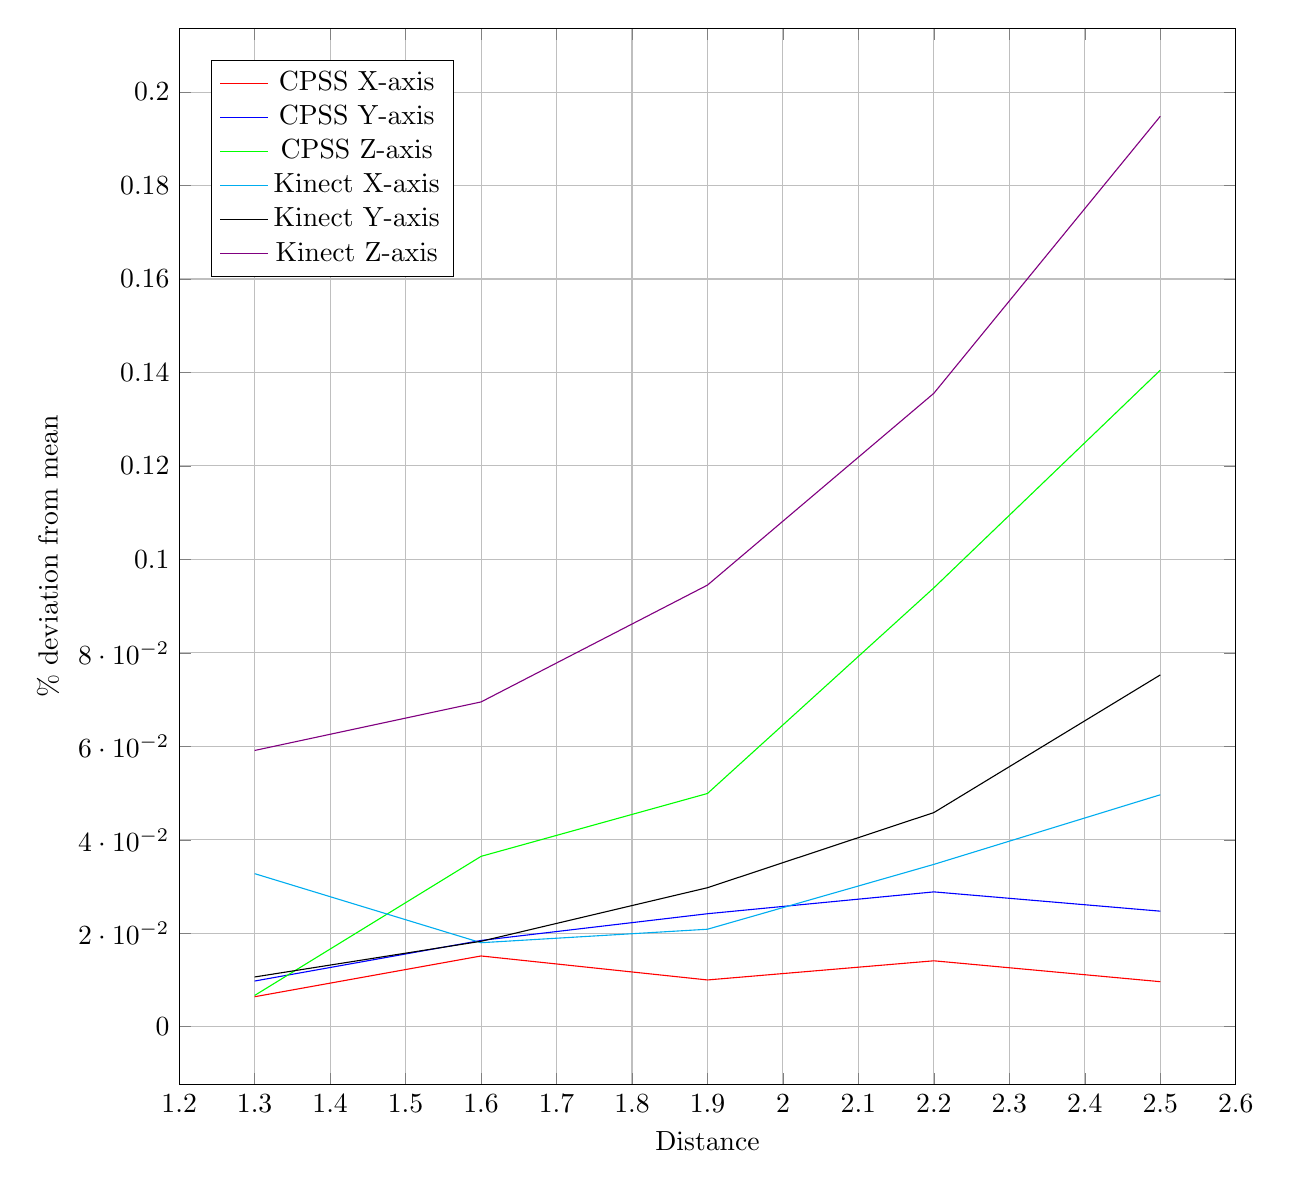
\begin{tikzpicture}
\begin{axis}[height=15cm,width=15cm,grid=major,xlabel=Distance,ylabel=\% deviation from mean,xmin=1.2,xmax=2.6,domain=1.2:2.6,legend entries={CPSS X-axis,CPSS Y-axis,CPSS Z-axis,Kinect X-axis,Kinect Y-axis,Kinect Z-axis},legend pos=north west]
%X-AXIS
\addplot [red] coordinates {(1.3,0.006418) (1.6,0.015143) (1.9,0.010009) (2.2,0.014109) (2.5,0.009640)}; %node [pos=0.1,pin={-10:$X$},inner sep=0pt] {};

%Y-AXIS
\addplot [blue] coordinates {(1.3,0.009779) (1.6,0.018461) (1.9,0.024181) (2.2,0.028856) (2.5,0.024728)}; %node [pos=0.3,pin={-10:$Y$},inner sep=0pt] {};

%Z-AXIS
\addplot [green] coordinates {(1.3,0.006695) (1.6,0.036458) (1.9,0.049911) (2.2,0.093916) (2.5,0.140487)}; %node [pos=0.6,pin={-10:$Z$},inner sep=0pt] {};


%Kinect data
%X-AXIS
\addplot [cyan] coordinates {(1.3,0.032756) (1.6,0.017977) (1.9,0.020863) (2.2,0.034741) (2.5,0.049633)}; %node [pos=0.2,pin={-10:$X$},inner sep=0pt] {};

%Y-AXIS
\addplot [black] coordinates {(1.3,0.010647) (1.6,0.018285) (1.9,0.029747) (2.2,0.045827) (2.5,0.075279)}; %node [pos=0.4,pin={-10:$Y$},inner sep=0pt] {};

%Z-AXIS
\addplot [violet] coordinates {(1.3,0.059115) (1.6,0.069500) (1.9,0.094501) (2.2,0.135550) (2.5,0.194821)}; %node [pos=0.7,pin={-10:$Z$},inner sep=0pt] {};


\end{axis}
\end{tikzpicture}
\caption{Distance versus precision along X,Y,Z axes}
\label{fig:dist_vs_prec}
\end{figure}
\noindent
Table 5-5 shows the dependence of measurement accuracy on distance for Kinect. Table 5-6 shows the dependence of measurement uncertainty on distance of measurement object from kinect sensor.

\begin{table}[ht]
\centering
\begin{tabular}{c c}
\hline\noalign{\smallskip}
Distance  & Kinect(\%  error) \\
\noalign{\smallskip}\hline\noalign{\smallskip}
1.3   & 1.194  \\
1.6   & 1.827  \\
1.9   & 1.911  \\
2.2   & 1.737  \\
2.5   & 1.057  \\
\noalign{\smallskip}\hline
\end{tabular}
\caption{Kinect:Dependence of measurement accuracy on distance}
\end{table}
\noindent

\begin{table}[ht]
\centering
\begin{tabular}{c c }
\hline\noalign{\smallskip}
Distance   & Kinect(\% uncertainty) \\
\noalign{\smallskip}\hline\noalign{\smallskip}
1.3    & 0.069 \\
1.6    & 0.191 \\
1.9    & 0.245 \\
2.2    & 0.261 \\
2.5    & 0.289 \\
\noalign{\smallskip}\hline
\end{tabular}
\caption{Kinect:Dependence of measurement uncertainty on distance}
\end{table}

\noindent
Although relative error in CPSS and Kinect doesn't gave a monotonous variation within the considered depth range but measurement uncertainty in kinect showed strict rise with increasing  distance from sensor. We can summarize these observations as average percentage relative error for CPSS was $\sim1.018\%$ while that for kinect was $\sim1.545\%$ within range of 1.3m-2.5m.Figure~\ref{fig:dist_vs_accuracy} represents the observed variation of measurement accuracy with distance, along with measurement uncertainty.

\begin{figure}[ht]
\centering
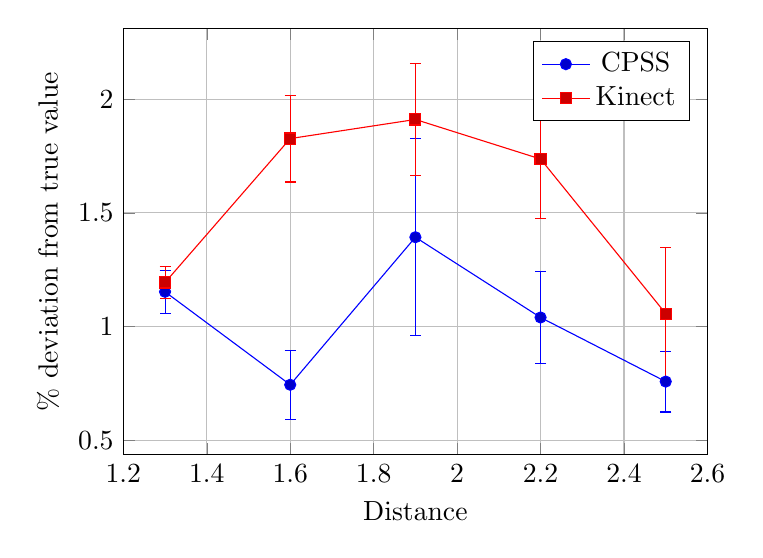
\begin{tikzpicture}
\begin{axis}[height=7cm,width=9cm,grid=major,xlabel=Distance,ylabel=\% deviation from true value,xmin=1.2,xmax=2.6,domain=1.2:2.6,legend entries={CPSS,Kinect},legend pos=north east]

\addplot +[blue,error bars/.cd,y dir=both,y explicit] coordinates {
(1.3,1.153) +- (0.0,0.095)
(1.6,0.744) +- (0.0,0.152) 
(1.9,1.393) +- (0.0,0.433)
(2.2,1.040) +- (0.0,0.204)
(2.5,0.758) +- (0.0,0.134)
};

\addplot +[red,error bars/.cd,y dir=both,y explicit] coordinates {
(1.3,1.194) +- (0.0,0.069)
(1.6,1.827) +- (0.0,0.191)
(1.9,1.911) +- (0.0,0.245)
(2.2,1.737) +- (0.0,0.261)
(2.5,1.057) +- (0.0,0.289)
};
\end{axis}
\end{tikzpicture}
\caption{Distance versus measurement accuracy with indication of uncertainty(vertical bars)}
\label{fig:dist_vs_accuracy}
\end{figure}






\subsection{Observations and conclusions}
\label{sec-4}
Kinect accuracy can be improved using system calibration[58][65][67][69].In our work we have used OpenNI default calibration parameters. Error-prone nature of both kinect and CPSS against surfaces with high reflectivity and very low reflectivity was observed. Further it was observed that due to disparity quantization multiple planes are visible in the scan of a single planar object and separation between these planes increases with increase in distance between object and sensor which was also reported by [63]. Here an approach is introduced for accuracy evaluation using 3D length measurements however deviations reported here may not be general statistics as [70] have observed different measurement accuracy for different units of kinect. Depth uncertainty in kinect is considerably higher than CPSS as shown in Tables 1 and 2. Although [71] reports relatively small improvement due to averaging over multiple measurements in range less than 3m, but it was found that the measurement uncertainty over 10 measurements was considerable(as shown in table 5.6) and should not be ignored, hence it suggests that averaging the measurements using multiple scans is important even within 2.5m.



\section{System calibration}
System calibration results in estimation of parameters which allow 3D sensor to map real-world 3D points defined in \textit{physical} units to 2D points defined in terms of \textit{pixels}. In this section, the tests performed to assess repeatability and accuracy of calibration algorithm are described. To assess repeatability, calibration was performed multiple times to determine \% average absolute deviation of estimated parameters from their mean values. For assessing accuracy, some \textit{reference} 3D points were selected whose 3D coordinates were known. These points were projected to camera/projector pixel coordinate space and the radial distance of projection from the \textit{observed} projection was considered as \textit{error}. A similar approach is described in [72]. The definition of \textit{system calibration error} $\varepsilon$ used in this work is described by the following equation:
\begin{equation}
\varepsilon=\frac{\sum_{i=1}^N\sqrt[2]{(X_t^i-X_e^i)^2+(Y_t^i-Y_e^i)^2}}{N}
\end{equation}
\noindent
$N$: Total 3D reference points used for testing system calibration parameters\newline
$(X_t^i,Y_t^i)$: True coordinates of 2D projection of $i^{th}$ reference point\newline
$(X_e^i,Y_e^i)$: 2D coordinates of $i^{th}$ reference point computed using system calibration parameters\newline

\subsection{Experiments and results}
Experiments to evaluate repeatability and accuracy of camera and projector intrinsic and extrinsic calibration parameters were performed. Procedure is already described in the parent section. For sake of brevity, equation 5.2 rephrases the relation used for projecting the $i^{th}$ reference point from real world 3D coordinates to 2D image coordinates in experiment for measuring accuracy of calibration parameters. Please refer section 2.1.2 for detailed explanation of this equation.
\begin{equation}
\begin{aligned}
& \begin{bmatrix}
U_e^i \\
V_e^i
\end{bmatrix} 
=A_c[R|T]\begin{bmatrix}
X_w^i \\
Y_w^i \\
Z_w^i
\end{bmatrix} \\
& \begin{bmatrix}
X_e^i \\
Y_e^i
\end{bmatrix}
=f(U_e^i,V_e^i)
\end{aligned}
\end{equation}
\noindent
where,\newline
$(X_w^i,Y_w^i,Z_w^i)$: 3D coordinates of $i^{th}$ reference point\newline
$(U_e^i,V_e^i)$: 2D undistorted coordinates of reference point in camera \newline
$A_c$: Camera intrinsic parameter matrix \newline
$[R|T]$: Camera extrinsic parameter matrix \newline
$f$: Camera distortion function estimated by calibration\newline
$(X_e^i,Y_e^i)$: 2D estimated coordinates of projection of reference point in camera image coordinate system\newline 
\noindent

\begin{enumerate}
\item{\textbf{Camera calibration}\newline}
In order to quantify the repeatability of the used OpenCV camera calibration algorithm which is an important measure of stability of any algorithm, we performed camera calibration 5 times and determined the \% average absolute deviation of its parameters. Table 5-7 shows the results.
\begin{table}[ht]
\centering
\begin{tabular}{c c}
\hline\noalign{\smallskip}
Parameter  & \% deviation \\
\noalign{\smallskip}\hline\noalign{\smallskip}
$f_x$   & 1.105  \\
$f_y$   & 1.075  \\
$c_x$   & 0.707  \\
$c_y$   & 0.894  \\
$k_1$   & 7.357 \\
$k_2$  &  8.825 \\
\noalign{\smallskip}\hline
\end{tabular}
\caption{Percentage average absolute deviation of camera calibration parameters}
\end{table}
\noindent
Results show considerably high uncertainty in estimating $k_1$ and $k_2$. This was observed for projector calibration as well(see table 5.9). So based on this test we can conclude that algorithm is repeatable within $\sim1\%$ for all parameters except distortion coefficients. Although more number of such tests can put more tighter and reliable limits.

Figure~\ref{fig:cam_calib_accuracy} shows the test scene with reference points which were used for estimating accuracy of calibration parameters. Coordinates of reference points were physically measured and used as \textit{true values}. Here true values were defined using corner-detection to detect image coordinates of reference points. Table 5-8 shows the result of projection of 3D points to camera image-space and their radial distance from corresponding \textit{observed} value. This test was repeatedly performed 5 times to reduce effect of random error in corner detection. 


\begin{figure}[ht]
\centering
\includegraphics[width=10cm,height=8cm]{../img_source/camera_calib_test.jpg}
\caption{Points A,B,C,D were used for measuring camera calibration accuracy}
\label{fig:cam_calib_accuracy}
\end{figure}






\begin{table}[ht]
\centering
\begin{tabular}{c c}
\hline\noalign{\smallskip}
Point  & Radial distance from true projection \\
\noalign{\smallskip}\hline\noalign{\smallskip}
A   & 2.553  \\
B   & 3.453  \\
C   & 4.080 \\
D   & 4.180 \\
\noalign{\smallskip}\hline
\end{tabular}
\caption{Camera calibration:Radial error of projection}
\end{table}
In table 5-8, radial error $\varepsilon$ points towards a systematic error since in all 5 measurements we observed that relation: $\varepsilon_{A}<\varepsilon_{B}<\varepsilon_{C}<\varepsilon_{D}$ holds, which demands further study.

\item{\textbf{Projector calibration}\newline}
During development it was observed that calibration parameters returned by OpenCV calibration algorithm for projector were not repeatable hence it was decided to use VPCLib[73] which gives considerably higher repeatability as shown in table 5-9.\newline
\indent
VPCLib assumes no distortion parameters in projector model. It estimates projector to 3D-plane homographies for multiple positions of projector with respect to plane. It further uses these homographies to compute points in 3D plane corresponding projector image points. Once these point correspondences are known it uses plane based calibration method for estimating the calibration parameters.  Further the estimated parameters are refined using \textit{Bundle adjustment} or non-linear minimization[73].\newline

\begin{table}[ht]
\centering
\begin{tabular}{c c c}
\hline\noalign{\smallskip}
Parameter  & OpenCV method & VPCLib method \\
\noalign{\smallskip}\hline\noalign{\smallskip}
$f_x$ & 7.625 & 2.166\\
$f_y$ & 7.445 & 2.047\\
$c_x$ & 5.559 & 1.795\\
$c_y$ & 4.381 & 1.861\\
$k_1$ & 38.196 & Not estimated\\
$k_2$ & 96.227 & Not estimated\\
\noalign{\smallskip}\hline
\end{tabular}
\caption{Percentage average absolute deviation of projector calibration parameters}
\end{table}
It can be clearly observed that VPCLib method gives much more repeatable results than OpenCV algorithm for projector calibration. Further it can observed that estimated $k_1$ and $k_2$ exhibit unacceptably high \% deviation. Hence VPCLib method was used for further analysis.\newline
\indent
As mentioned above, VPCLib method do not assume distortion parameters in projector model since projectors practically have negligible radial distortion hence $k_1$ and $k_2$ were not estimated and were assumed to be 0.\newline
To assess accuracy of projector intrinsic and extrinsic parameters estimated by VPCLib, 3D coordinates of corners of projection on a plane were determined through physical measurement and then they were reprojected back to projector image. Figure~\ref{fig:proj_calib_accuracy} shows the projected blank image whose corners were used for accuracy assessment. Radial distance between \textit{true} image coordinates and coordinates estimated through calibration parameters was considered as \textit{error}. Table 5-10 shows the deviation between observed and estimated 2D projector coordinates. Here again we observe a pattern in radial error in which error is monotonically increasing from point A to point D which is similar to that was observed in case of camera calibration in table 5-8.
\begin{figure}
\centering
\includegraphics[width=10cm,height=8cm]{../img_source/proj_calib_test.jpg}
\caption{Corners A,B,C,D were used for assessing accuracy of projector calibration parameters}
\label{fig:proj_calib_accuracy}
\end{figure}

\begin{table}[ht]
\centering
\begin{tabular}{c c}
\hline\noalign{\smallskip}
Point  & Radial distance from true projection \\
\noalign{\smallskip}\hline\noalign{\smallskip}
A   &  6.776 \\
B   &  8.608 \\
C   &  11.728\\
D   &  18.248\\
\noalign{\smallskip}\hline
\end{tabular}
\caption{Projector calibration:Radial error of projection}
\end{table}
\end{enumerate}

\subsection{Limitations of the used testing method}
This approach requires us to define \textit{true} 3D reference coordinates which is not practical at larger distances from reference origin without using a CMM machine or any other highly accurate metrology equipment. Hence this approach do not allow to practically cover entire \textit{calibration volume} to define accuracy of calibration parameters in general. Hence there is a need of an \textit{automated} method which can efficiently cover entire calibration volume without any requirement of manual intervention to define true values for 3D reference points. Even for exhaustive testing at distance where true 3D coordinates can be conveniently measured it is very time consuming process. Further to define $(X_t^i,Y_t^i)$ we need to use a \textit{feature detector} which in itself will add corner detection errors.  



\section{Stereo correspondence}
Stereo-correspondence relates pixels in camera and projector image which corresponds to a common point in real world. To assess accuracy of stereo-correspondence achieved using coded phase shift technique a \textit{known} checkerboard pattern was projected. Corners of checkerboard were detected and corresponding projector coordinates were determined using the stereo-correspondence estimated using coded phase shift technique. Accuracy is defined to be the \textit{radial} distance of estimated projector coordinates for detected checkerboard corners from the true coordinates of the checkerboard corners in projector image. The definition of \textit{stereo-correspondence error} used in this work is described by the following equation:
\begin{equation}
\varepsilon=\frac{\sum_{i=1}^N\sqrt[2]{(X_t^i-X_e^i)^2+(Y_t^i-Y_e^i)^2}}{N}
\end{equation}
\noindent
where,\newline
$N$: Total number of checkerboard corners used for testing stereo-correspondence \newline
$(X_t^i,Y_t^i)$: True coordinates of $i^{th}$ checkerboard corner\newline
$(X_e^i,Y_e^i)$: Estimated coordinates of $i^{th}$ checkerboard corner

\subsection{Experiments and results} 
Stereo-correspondence for a phase-shift technique is mainly affected by non-linear output response of projection and capture devices to the applied input[7][42]. This non-linearity can be compensated by a factor called \textit{gamma}. Projector Gamma allows manipulation of contrast of projected image such that non-linearity of input-to-output behavior of projector can be compensated. Furthermore a projected sinusoidal pattern can \textit{appear} non-sinusoidal if contrast of projected image has not been controlled to suppress non-linearity of device. Although same holds for camera also but in this work we have limited our scope to study the effects of projector gamma.\newline
\indent
Incorrect value of gamma leads to apparent \textit{waviness} in the 3D reconstructions as shown in figure~\ref{fig:gamma_3_phase} which shows the zoomed view of reconstruction of a planar object for different values of gamma. Here $\gamma=2.041$ seems to be more accurate gamma value since planarity of reconstructed surface is higher than that for $\gamma=1.0$.
\begin{figure}[htbp]
\def\tabularxcolumn#1{m{#1}}
\begin{tabularx}{\linewidth}{@{}cXX@{}}
\begin{tabular}{c c}
\subfloat[$\gamma=1.0$]{\includegraphics[width=7cm,height=7cm]{../img_source/3_phase_1_test_2.jpg}} & 
\subfloat[$\gamma=2.041$]{\includegraphics[width=7cm,height=7cm]{../img_source/3_phase_2_041_test_2.jpg}}\\
\end{tabular}
\end{tabularx}
\caption{Effect of gamma on 3D reconstruction of a plane}
\label{fig:gamma_3_phase}
\end{figure}
Clearly this will affect the measurement accuracy of the system. So the target in this work was to study the effect of projector gamma on stereo-correspondence error.\newline
\indent Further, in literature it has been reported that effect of non-linearity reduces with increasing number of phase shifted patterns used to acquire stereo-correspondence[7]. This can be observed in figure~\ref{fig:gamma_3_4_5} which shows reduction in \textit{waviness} in zoomed view of reconstruction of a planar object using 4 and 5 phase shifted patterns as compared to 3 phase shifted patterns. Hence,it was further attempted to quantify the effect of number of phase shifted patterns on stereo-correspondence error.
\begin{figure}[ht]
\def\tabularxcolumn#1{m{#1}}
\begin{tabularx}{\linewidth}{@{}cXX@{}}
\begin{tabular}{c c}
\subfloat[3 phase]{\includegraphics[width=7cm,height=7cm]{../img_source/phase_3_edit.jpg}} &
\subfloat[4 phase]{\includegraphics[width=7cm,height=7cm]{../img_source/phase_4_edit.jpg}}\\
\subfloat[5 phase]{\includegraphics[width=7cm,height=7cm]{../img_source/phase_5_edit.jpg}} \\
\end{tabular}
\end{tabularx}
\caption{Effect of increasing number of phase shifted patterns on \textit{waviness} in 3D reconstruction}
\label{fig:gamma_3_4_5}
\end{figure}
\FloatBarrier
\noindent Tests as already described in the parent section were performed for both cases i.e., varying gamma for 3 phase shifted pattern approach and by varying the number of projected phase-shifted fringe patterns under a constant gamma($\gamma=1$). Table 5.11 shows the effect of projector gamma on stereo-correspondence error. Table 5.12 shows the effect of increasing number of phase-shifted patterns on stereo-correspondence error.   

\begin{table}[htbp]
\centering
\begin{tabular}{c c}
\hline\noalign{\smallskip}
Gamma($\gamma$)  & Stereo-correspondence error \\
\noalign{\smallskip}\hline\noalign{\smallskip}
1.0   &  1.890\\
1.524   &  1.682 \\
1.912   &  1.730\\
2.041   &  1.588\\
2.559 & 2.073\\
2.947 & 2.394\\
\noalign{\smallskip}\hline
\end{tabular}
\caption{Stereo-correspondence error for various gamma values for 3 phase-shifted method}
\end{table}

\begin{table}[htbp]
\centering
\begin{tabular}{c c}
\hline\noalign{\smallskip}
Number of patterns  & Stereo-correspondence error \\
\noalign{\smallskip}\hline\noalign{\smallskip}
3   &  1.890 \\
4   &  2.100 \\
5   &  2.454\\
\noalign{\smallskip}\hline
\end{tabular}
\caption{Stereo correspondence error for 3,4,5 phase shifted patterns}
\end{table}
\noindent


In table 5.11 it can be observed that there is reduction in stereo-correspondence error from $\gamma=1.0$ to $\gamma=2.041$ followed by increase monotonous increase in error from $\gamma=2.559$. But in table 5.12 we got contradictory results to our expectation. To further confirm this observation we performed experiment 5 times but same pattern of monotonous increase in correspondence error from 3 to 5 phase shifted patterns was observed. This highlights the shortcomings of used criteria for stereo-correspondence error. Although criteria is correct in its formulation because if increasing number of phase-shifted patterns reduces effect of system non-linearity as has been observed in figure~\ref{fig:gamma_3_4_5} then it must result in reduction in stereo-correspondence error as defined here. It encourages for further study on how to apply this criteria correctly. 

\subsection{Limitations of the used testing method}
This approach works as long as projected features can be uniquely recognized so that explicit correspondence estimation for the reference pattern features itself is not required. This can be conveniently used for assessing stereo-correspondence errors in case of a planar scene with no occlusions, since correspondence between camera and projector for feature points in the reference pattern can be easily established. But for complex surfaces with surface discontinuities, curvature, where correspondence between camera and projector for reference pattern cannot be implicitly assumed we either have to use any other technique to define correspondence for the features or an altogether different approach to test stereo-correspondence. Further, accuracy of feature detection will also affect the computed correspondence error.


\section{Triangulation}
Triangulation as described in chapter-4 computes 3D coordinates of a real-world point given stereo-correspondence between camera-projector and system calibration parameters. Although it is already mentioned that accuracy evaluation of optical triangulation cannot be done reliably unless we have exact quantitative error bounds for calibration and correspondence for any test case, it is possible to compare different triangulation methods with respect to the accuracy of estimated 3D coordinates of any feature in the scene without changing correspondence and system calibration parameters in the process. This approach do not require us to have knowledge about \textit{exact} error bounds of correspondence and calibration. Hence it is proposed to define \textit{triangulation error} as the deviation of estimated 3D coordinates of a feature in the scene with respect to that reported by CMM machine. Here coordinate measurement is proposed rather than conventional dimension measurement since coordinate measurement indirectly reflects accuracy of dimensions.








\section{Summary}
In this chapter, the approaches used for assessing accuracy of stereo-correspondence and system calibration parameters was described along with the limitations of such approaches. Furthermore, a test was proposed to evaluate accuracy of optical triangulation which was not in the scope of work due to time limitations.\newline
\indent In addition, comparison of measurement accuracy and precision of developed system with Microsoft Kinect has been described. Here we examined reconstruction accuracy in static scenes and observed that within depth range of 1.3m-2.5m(based on combine depth-of-field of camera projector system) kinect reconstructs with ~0.5 percent higher relative error as compared to CPSS, further the precision of 3D data generated by both techniques using reconstruction of a planar object at various distances was analyzed, and it was observed that for both kinect and CPSS, there is a strong relationship between distance of object from sensor and uncertainty in measurement. Overall CPSS exhibits relatively lower uncertainty in X,Y,Z, coordinates. Furthermore it was observed that CPSS has almost equal uncertainties in X,Y,Z coordinates but kinect exhibits considerably higher uncertainty along Z-axis(depth-uncertainty) as compared to that along X and Y axes.

 
